\documentclass[11pt]{article}
\usepackage[utf8]{inputenc}
\usepackage{amsmath}
\usepackage{amssymb}
\usepackage{graphicx}
\usepackage{hyperref}
\usepackage[parfill]{parskip}
\let\oldemptyset\emptyset
\let\emptyset\varnothing


\title{\textbf{Esssentials of Applied Data Analysis\\
				IPSA-USP Summer School 2017}\newline\\
				Sample, Confidence Intervals and Hypothesis testing in Classical Statistics}

\author{Leonardo Sangali Barone\\ \href{leonardo.barone@usp.br}{leonardo.barone@usp.br}}
\date{jan/17}

\begin{document}

\maketitle
\section{Sample and sample distribution of parameters.}

	\subsection*{CLT and sampling}
	
	Central Limit Theorem: if we take enough samples from our population, whose mean of one characteristic of the population (age, income, etc) is $\mu$, and observe the distribution of all of the samples means ($\bar{X}$), the distribution of the sample means is assimptotically (in the infinite) normal (if, of course, CLT assumptions hold).\\

	Let's take a closer look at the sample and sample distribution of the mean.\\
	
	Remember: the sample distribution of the mean (of one characteristic of the population) is different from the distribution of the characteristic in the sample

	\subsection*{Population \emph{versus} sample}
	First, let's take a look at the parameters of the population and the sample.\\

\begin{figure}[htp]
\centering
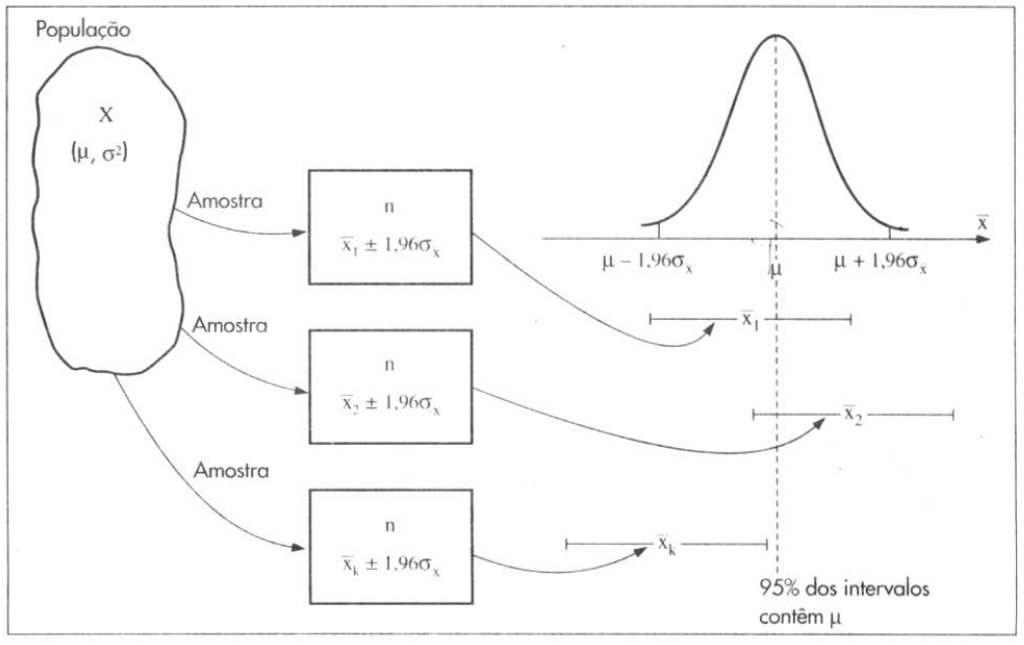
\includegraphics[scale=0.60]{bci.png}
\caption{Sampling proccess}
\label{}
\end{figure}

\begin{tabular}{|c|c|c|}
\hline
	Parameter & Population & Sample estimate\\ 
\hline
	Mean & $\mu$ & $\hat{\mu} = \bar{x} = \frac{1}{n}\sum\limits_{i=1}^n x_i $\\
	Variance & $\sigma^2$ & $\hat{\sigma}^2 = s^2 = \frac{1}{n-1}\sum\limits_{i=1}^n (x_i - \bar{x}) $\\
\hline
\end{tabular}

With the sample formulas we can obtain an estimate of the parameters of the population ($\hat{\mu}$ and $\hat{\sigma}^2$ are our best guess of what the population mean and population variance are).

	\subsection*{Population \emph{versus} sample - proportion}
	In some cases, we are interested in the sample estimation of a proportion, whose notation and formulas cab ne found below.\\

\begin{tabular}{|c|c|c|}
\hline
	Parameter & Population & Sample estimate\\ 
\hline
	Proportion & $p$ & $\hat{p}$\\
	Variance & $\sigma^2 = p*(1-p)$ & $\hat{\sigma}^2 = s^2 = \hat{p}*(1-\hat{p})$\\
\hline
\end{tabular}
\newline\\



	\subsection*{Sample distribution of a parameter}

Good, we already know the mean and variance of a variable in the population and in a sample. Now, what is the \textbf{variance of the sample mean}? Can you see how trick this question is? Let's call this variance $\sigma_{\bar{x}}^2$ (sigma square of x-bar).\\
	
	The variance and standard deviation of the sample mean ($\sigma_{\bar{x}}^2$) is simply this:
\[\sigma_{\bar{x}}^2 = \frac{\sigma^2}{n} \text{ and }\sigma_{\bar{x}} = \frac{\sigma}{\sqrt{n}}\]
Where $n$ is the sample size.

	\subsection*{Sample distribution of a parameter - HDI}

Example: There are 5560 (aprox.) municipalities in Brazil. We know (because we have data of the universe of municipalities) that the mean HDI (Human Development Index) of that set of municipalities in 2000 was aproximately $\mu_{HDI}=0.69$ and the standard deviation $\sigma_{IDH} = 0.08$. If we take a random sample of 100 municipalities and observe the sample mean ($\bar{x}$) what is the standard deviation of the sample mean ($\sigma_{\bar{x}}$)?

\[\sigma_{\bar{x}} = \frac{\sigma_{IDH}}{\sqrt{n}} = \frac{0.08}{\sqrt{100}} = \frac{0.08}{10} = 0.008\]

In our example, we already know what is the population standard deviation, so we can do

\[\sigma_{\bar{x}}^2 = \frac{\sigma^2}{n}\]

What if we don't have the population standard deviation? In large random samples, we can use the sample estimate of the standard deviation as a substitute.

\[\hat{\sigma}_{\bar{x}}^2 = \frac{\hat{\sigma}^2}{n} \text{  or  } s_{\bar{x}}^2 = \frac{s^2}{n}\]

	\subsection*{Sample distribution of a parameter - proportion}

	If we are interested in a proportion instead of a mean, then the \textbf{variance of the sample proportion $\hat{p}$ is}:

\[\sigma_{\hat{p}}^2 = \frac{\sigma^2}{n} = \frac{\hat{p} * (1-\hat{p})}{n} \text{ and }\sigma_{\hat{p}} = \frac{\sigma}{\sqrt{n}} = \sqrt{\frac{\hat{p} * (1-\hat{p})}{n}}\]

where $n$ is the sample size.


	\subsection*{Bigger n}

	On daily reaserch pratice, we are often worried about the size of our sample? Why is that?\\

	Because the larger the sample, the smaller the standard deviation of our estimates and the large is the confidence we got the right number.\\
	
	Let's see what happens with the distribution of the sample mean in our example of Brazilian municipalities.



	\subsection*{Standardization}
	Before we move to estimation and hypothesis testing, let's learn how to standardize values in the normal distribution.\\
	
	We know that the normal curve depends on two values: $\mu$ and $\sigma$, it's mean and standard deviation. To standardize a value means to locate it at one special normal distribution, the $Z$ curve, which is the normal with $\mu =0 $ and $\sigma =1$\\

	The standardization process of a value x is quite simple:

	\[z=\frac{x - \mu}{\sigma}\]

	Intuitively, we are "centering" our distribution in the 0 by subtracting $\mu$ and making the standard deviation to became a unit by dividing by $\sigma$ 


\section{Confidence intervals}

	\subsection*{Estimation}
\emph{Point estimate}: A single statistic value that is the “best guess” for
the parameter value.\\

\emph{Interval estimate}: An interval of numbers around the point estimate, that has a fixed “confidence level” of containing the parameter value. Called a confidence interval. (Based on sampling distribution of the point estimate).\\

	Intuitively, confidence intervals are the "range" of values in which the real population parameter is very likely to be (when we don't know the population parameter and we want to learn about it).

	\subsection*{Confidence interval}
	
	\emph{First step:}\\
	
	How to build a confidence interval? First, we take the sample estimate of the paramater. If we want to know the population mean ($\mu$), than we take the population sample ($\bar{x}$). If we want to know the population proportion $p$, then we take the $\hat{p}$.\\

	\emph{Second step:}\\

	We define a level of confidence ($\gamma$), let's say, $95\%$. By choosing a level of condifence we are saying that if we sample from our population multiple times, in $95\%$ of the times the population parameter will fall in my interval.\\
	
	We locate on the $Z$ curve the interval, centered at $0$ whose probability is $0.95$. This inteval is $[-1.96;1.96]$. We call the limits of the interval critical values ($z_\gamma$) .

	\emph{Final step:}\\

	We do the oposite of the standardization process. We multiply this interval we found at the $Z$ curve by the standard deviation of the sample mean ($s_{\bar{x}}$ or $\hat{\sigma}_{\bar{x}}$ and we center it at the sample mean. Our interval with $\gamma = 95\%$ level of confidence is:
	\[[\bar{x}-z_\gamma*\hat{\sigma}_{\bar{x}};\bar{x}+z_\gamma*\hat{\sigma}_{\bar{x}}] = [\bar{x}-1.96*\hat{\sigma}_{\bar{x}};\bar{x}+1.96*\hat{\sigma}_{\bar{x}}]\]

\begin{figure}[htp]
\centering
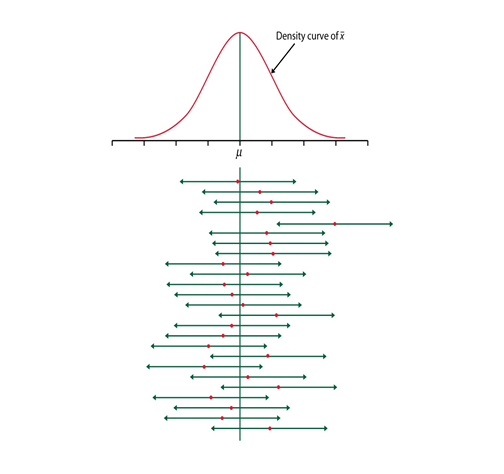
\includegraphics[scale=1.00]{ci.png}
\caption{Confidence Intervals}
\label{}
\end{figure}

	\subsection*{Confidence interval - proportion}
	
	The confidence interval for proportions looks very similar to the confidence interval for the mean, as long as you do the appropriate substitutions:
	
	\[[\hat{p}-z_\gamma*\hat{\sigma}_{\hat{p}};\hat{p}+z_\gamma*\hat{\sigma}_{\hat{p}}]=[\hat{p}-1.96*\hat{\sigma}_{\hat{p}};\hat{p}+1.96*\hat{\sigma}_{\hat{p}}]\]

	\subsection*{Confidence interval}
	
	Look at the $Z$ table you have been given. What happens if you choose a greater level of confidence, for example, $99\%$? What if you choose a lesser level of confidence, for example, $90\%$?\\

The confidence interval is itself a random quantity, subject to sampling variability.\\

In the “long run,” $95\%$ of the confidence intervals for a population mean $\mu$ will actually cover $\mu$

	\subsection*{Errors and sample size}

	Look again at the confidence interval.

	\[[\bar{x}-z_\gamma*\hat{\sigma}_{\bar{x}};\bar{x}+z_\gamma*\hat{\sigma}_{\bar{x}}]\]

	Let's define an error $\epsilon$ as:
	
	\[\epsilon=z_\gamma*\hat{\sigma}_{\bar{x}}\]	
	
	And let's substitute the standard deviation of the sample mean, $\hat{\sigma}_{\bar{x}}$, by it's original formula:
	
	\[\epsilon=z_\gamma*\frac{\hat{\sigma}}{\sqrt{n}}\]	

Now, imagine that we want to define the maximum error ($\epsilon$) we want and we want to choose a certain level of confidence (which determines $z_\gamma$). Since we don't have any control of the standard deviation of the population ($\sigma$), what we have to do is to get a population size ($n$) that safisties our restrictions (maximum standard error and level of confidence).

	\[\epsilon=z_\gamma*\frac{\sigma}{\sqrt{n}} => n=\frac{\sigma^2*z_\gamma^2}{\epsilon^2}\]	

\section{Hypothesis testing}


	With a good knowledge of how the normal curve is built, sampling e confidence intervals we can now test hypothesis.\\
	
	We are going to see today only the mean hypothesis testing. If we get the intuition correctly, any other test is easy\\
	
	We also call hypothesis testing as significance tests.

	We can generally think in 3 different objectives for hypothesis testing, depending on what we know about the population(s).
	\begin{itemize}
		\item If we know something about the population (mean and variance), we might want to know if a random sample actually comes from that population (and not from some other population);
		\item If we don't know anything about the population, we might to learn something (example: mean) or we might want to see if it is equal to our theory/prior belief;
		\item And finally (and that is more usefull in social sciences) we might want to compare two populations (groups!) and see if they are equal.
	\end{itemize}

	\subsection*{Null Hypothesis}

	\begin{itemize}
		\item If we know something about the population (mean and variance), we might want to know if a random sample actually comes from that population (and not from some other population)
		\[H_0: \mu = \text{population mean}\]
		\item If we don't know anything about the population, we might to learn something (example: mean) or we might want to see if it is equal to our theory/prior belief. Zero is a commom value to be tested.
		\[H_0: \mu = \text{hypothetical value} \]
		\item Finally (and that is more usefull in social sciences) we might want to compare two populations (groups!) and see if they are equal.
		\[H_0: \mu_{diff} = \mu_1 - \mu_2 = 0\]
	\end{itemize}


	\subsection*{Hypothesis testing - important}
	\begin{itemize}
		\item Your null hypothesis ($H_0$) is the one to be rejected.
		\item Your null hypothesis is the one that has the $=$ symbol. You can say that it is different by rejecting that it's equal, but not the opposite.
		\item If you can do with the sample mean, you can do with the sample proportions. Just substitute $\mu$ for $p$, $\bar{x}$ for $\bar{p}$ and $\hat{\sigma}_{\bar{x}}$ for $\hat{\sigma}_{\hat{p}}$.
		\item If you are comparing two populations, than you best counterfactual is zero difference. If you are testing dependence, then your best counterfactual is independence. If you are looking for a pattern, then randomness is your counterfactual.
	\end{itemize}

	\subsection*{Hypothesis testing - $Z$ or $t$?}
	You will see that for sifnificance tests we will use t-statistics. Remember that for samples over 30 observations it doesn't really matter in pratice which one to use. If you don't know which one to use, ask yourself
	\begin{enumerate}
		\item Do you know the population variance? If not, use $t$.
		\item Do you have more than 30 observations? If not, use $t$.
		\item You can use $Z$ if you answered yes to both questions.
	\end{enumerate}


	\subsection*{Hypothesis testing - mechanics}
	\begin{enumerate}
		\item Build your hypothesis
		\item Choose a level of significance, $\alpha = 1 - \gamma$, where $\gamma$ is the level of confidence
		\item "Take" your estimated value to the t curve/normal curve by standardazing it. The result will be the $t$ statistics or $z$ statistics:

		\[t = \frac{\bar{x} - \mu}{\hat{\sigma}_{\bar{x}}} \text{ or } z = \frac{\bar{x} - \mu}{\sigma_{\bar{x}}}\]

		$\mu$, for all purposes, is the value in the null hypothesis. 
	\end{enumerate}

	\subsection*{Hypothesis testing - mechanics for proportions}

	Substitute $\mu$ for $p$, $\bar{x}$ for $\bar{p}$ and $\hat{\sigma}_{\bar{x}}$ for $\hat{\sigma}_{\hat{p}}$ and you have the proportions test.

		\[t = \frac{\hat{p} - p}{\hat{\sigma}_{\hat{p}}} \text{ or } z = \frac{\hat{p} - p}{\sigma_{\hat{p}}}\]


	\subsection*{Hypothesis testing - two populations}
	When we test the difference between the mean of two samples, there two possible situations. In one, we know the population variance and we also know that both samples come from that population (\emph{equal variances}). Usually, however, we don't know that and we also know that they come from different populations. In those cases, we have to obtain the variance of the difference estimator, $\bar{x}_{diff} = \bar{x}_1 - \bar{x}_2$, which is:
	
	\[\hat{\sigma}^2_{\bar{x}_{diff}} = \hat{\sigma}^2_{\bar{x}_1 - \bar{x}_2} = \frac{\hat{\sigma}^2_{\bar{x}_1}}{n_1}+ \frac{\hat{\sigma}^2_{\bar{x}_2}}{n_2}\] 

	The same holds for proportion tests of two populations.


\end{document}
